\section{Aplicación de ejemplo}
Para ilustrar el uso de las herramientas desarrolladas utilizaremos como ejemplo
una aplicación bancaria, en la que los clientes de un banco pueden transferir
dinero de una cuenta a otra. 
Realizar una transferencia implica extraer el
monto indicado de una cuenta, y depositarlo en otra. 
Al ejecutar cualquiera de estas dos operaciones se pueden producir errores,
como por ejemplo, que no haya saldo saldo suficiente, o que el depósito supere
el máximo permitido.
La figura \ref{example} muestra las clases que implementan la lógica del
dominio.

	\begin{figure}[h!]
		\centering
		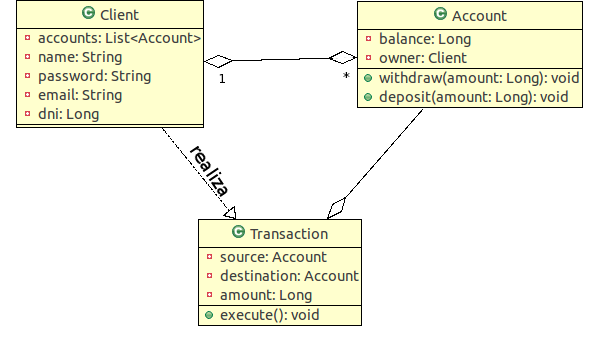
\includegraphics[width=500px, height=285px]{img/transaccion}
		\caption{Diagrama UML de la aplicación de ejemplo}
		\label{example}
	\end{figure}	

A continuación se describirán las dos pantallas más importantes de la
aplicación, que nos permitirán mostrar las diferentes utilidades brindadas por
nuestra propuesta.
 
\subsection{Transferencia simple} 
	Tres ventajas:
	- queda más simple
	- menos posibilidad de mandármela
	- concurrencia.

La figura \ref{executeTransaction} muestra el método  \lstinline|execute| de la
clase \lstinline|Transaction| \begin{figure}[h]
	\begin{lstlisting}
		public void execute(){
			this.source.withdraw(this.amount);
			this.destination.deposit(this.amount);
		}
	\end{lstlisting}
	\caption{Fragmento de código de la Clase Transaction}
	\label{executeTransaction}
\end{figure}
  	
\subsection{Transferencias múltiples}
	muchas transferencias en una única transacción\ldots fijate si sale algo y si no
	lo volamos.

